%!TEX root = ../TTT4150-Summary.tex
\section{GPS coordinate frames, time reference, and orbits}

%%%%%%%%%%%%%%%%%%%%%%%%%%%%%%%%%%%%%%%%%%%%%%%%%%%%%%%%%%%%
\subsection{Global coordinate systems}

\subsubsection{Conventional terrestrial reference system (CTRS)}
The \emph{pole of rotation} moves relative to the true pole. The \emph{Conventional terrestrial pole} (CTP) is a defined position corresponding to the average position of the pole of rotation between 1900 and 1905. With this, CTRS is defined with
\begin{itemize}
    \item origin at Earth mass center,
    \item $z$-axis through the CTP,
    \item $x$-axis through the intersection of CTP's equatorial plane and a reference meridian, and
    \item $y$-axis to complete a right-handed system.
\end{itemize}

In practice, this is implemented as the coordinate system that best fits a number of reference points with assigned coordinates.

\subsubsection{Conventional inertial reference system (CIRS)}
An inertial frame is nonaccelerating. CTRS spins with the Earth, and is therefore not inertial. Defined with
\begin{itemize}
    \item origin at Earth mass center,
    \item $z$-axis along the axis of rotation,
    \item $x$-axis in the equatorial plane, toward the vernal equinox,
    \item $y$-axis to complete a right-handed system.
\end{itemize}

\subsubsection{International terrestrial reference frame (ITRF)}
More accurate realization of CTRS than WGS 84 ECEF, used for research. Defined from a large number of reference stations around the world.

\subsubsection{WGS 84}
A realization of CTRS. It defines
\begin{itemize}
    \item an ECEF Cartesian coordinate frame,
    \item an ellipsoid model of the Earth,
    \item a characterization of Earth's gravity field and geoid, and
    \item some constants.
\end{itemize}
and its parameters are:
\begin{itemize}
    \item Semi-major axis $a$
    \item Reciprocal flattening $\frac{1}{f}$
    \item Earth's angular velocity $\omega_E$
    \item Earth's gravitational constant $GM$
    \item Speed of light in vacuum $c$
\end{itemize}

%%%%%%%%%%%%%%%%%%%%%%%%%%%%%%%%%%%%%%%%%%%%%%%%%%%%%%%%%%%%
\subsection{GPS orbits}

\begin{figure}[htbp]
    \centering
    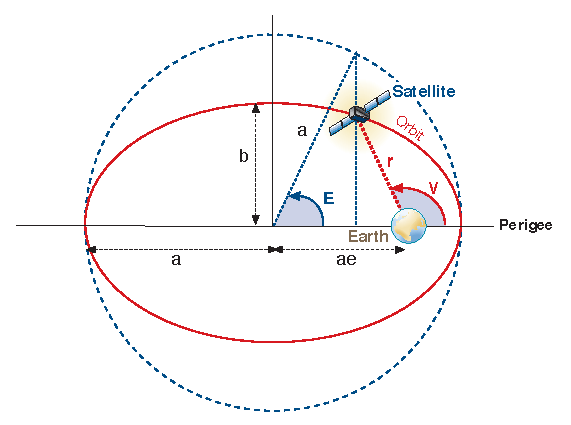
\includegraphics[width=\linewidth]{img/satellite-anomalies.pdf}
    \caption{True anomaly $V$ and eccentric anomaly $E$}
    \label{fig:orbital-anomalies}
\end{figure}



\subsubsection{Kepler's laws}
The laws are modified for satellites orbiting Earth.

\begin{enumerate}
    \item The satellite orbit is an ellipse with Earth at one focus.
    \item The line between the satellite and Earth sweeps over equal areas during equal intervals of time. (I.e. faster close to Earth.)
    \item The square of the orbital period is proportional to the cube of the semi-major axis of the orbit: $T^2 \propto a^3$
\end{enumerate}



\subsubsection{Keplerian elements}

\begin{figure}[htbp]
    \centering
    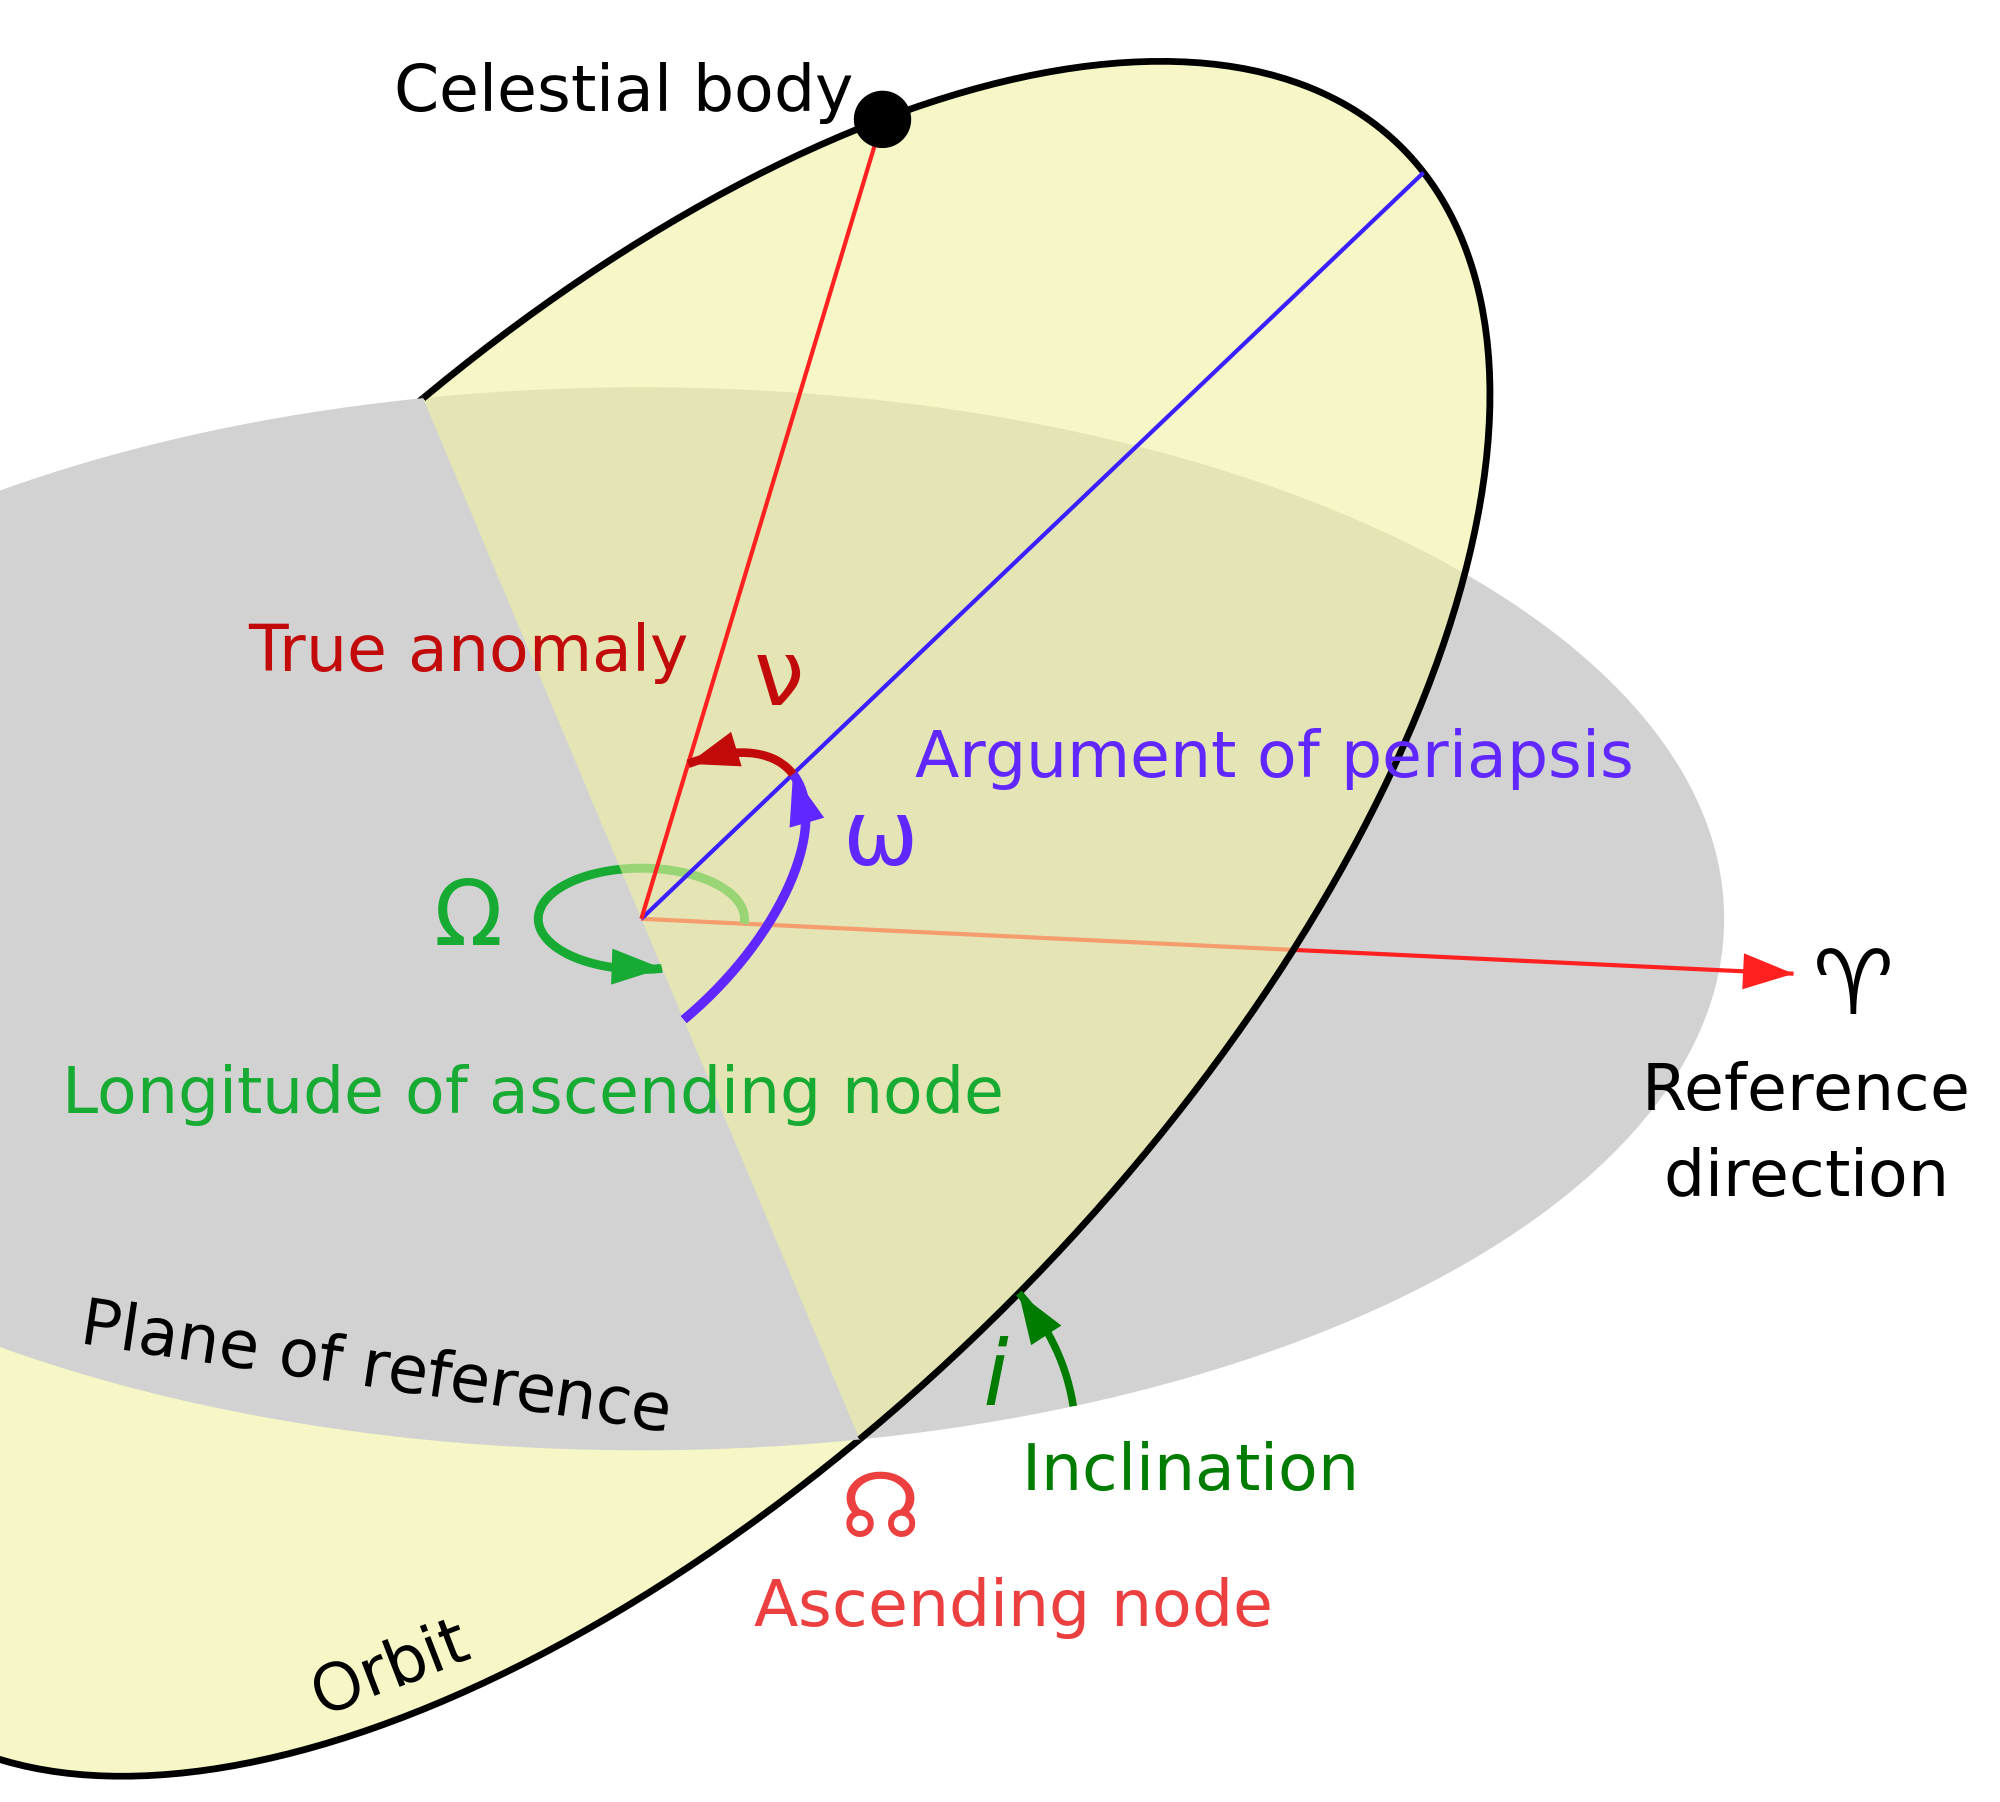
\includegraphics[width=.9\linewidth]{img/kepler-elements.png}
    \caption{Some Kepler elements, expressed generally, not terrestrially}
    \label{fig:kepler}
\end{figure}

The Keplerian elements are given at a specific epoch, and are as follows:

\begin{enumerate}
    \item[$a$]
        \textbf{Semi-major axis} $a$: Length of the semi-major axis of the elliptical orbit.
    \item[$e$]
        \textbf{Eccentricity} $e$: The eccentricity of the elliptical orbit.
    \item[$i$]
        \textbf{Orbital inclination} $i$: The orbital plane intersects the Earth center, but usually at an angle relative to the equator. This angle is the inclinaton.
    \item[$\Omega$]
        \textbf{Right ascension of the ascending node} $\Omega$: First: The intersection between the equator and the orbital plane is called the line of nodes. The nodes are the two points where the line intersects the surface. The ascending node is the node above which the satellite ascends (passes in a south to north direction).

        The RAAN is then the angle from the direction of the vernal equinox to the ascending node. The vernal equinox is a fixed point in the sky above equator, not rotating with Earth. (The vernal equinox is actually the ascending node of the Sun, meaning the sun has $\Omega = 0$.)

        In Figure \ref{fig:kepler}, it is called ``longitude of ascending node''.
    \item
        \textbf{Argument of perigee} $\omega$: The perigee is the point of the orbit closest to Earth. The argument of perigee is the angle between the ascending node and the perigee, as seen from Earth.

        In Figure \ref{fig:kepler}, this is called ``argument of periapsis''.
    \item
        \textbf{True anomaly} $\nu$: The angle between the perigee and the satellite, as seen from Earth.
\end{enumerate}



\subsubsection{Satellite position and velocity}

The orbital plane is specified fully by $a$, $e$, $i$, $\Omega$, and $\omega$ defined above. If we know $\nu$ at an epoch, we can find the position at any given time. In addition to \emph{true} anomaly $\nu$, we have \emph{eccentric} anomaly and \emph{mean} anomaly are defined:
\begin{itemize}
    \item
        \textbf{Eccentric anomaly} $E$: The angle between the perigee and the projection of the satellite onto a circle of radius $a$, as seen from the center of the orbit. See angle ``E'' in Figure \ref{fig:orbital-anomalies}.
    \item
        \textbf{Mean anomaly} $M$: The angle between the perigee and the place the satellite would have been had it been on a circular orbit with the same focus and period. See angle ``M'' in Figure \ref{fig:orbital-anomalies}.
\end{itemize}

\paragraph{Kepler's equation}
$E$ and $M$ are related by \emph{Kepler's equation}:
\begin{equation}
    M = E - e \sin E
\end{equation}



\subsubsection{Perturbations}
\emph{Precession} (period \SI{25800}{years}) and \emph{nutation} (\SI{18.6}{years}) affect satellite orbits.
